% En esta seccion se presentan experimentos concretos efectuados, exitosos o fallidos, mediante figuras y capturas de pantalla debidamente tituladas y referenciadas en el cuerpo del reporte.

\section{Experimentos}

\subsection{Actividad 1: Modelado de una pierna con articulaciones jerarquizadas en Blender}

Iniciamos el experimento modelando la pierna como una sola malla continua a partir de un cilindro primitivo en Modo Objeto (\texttt{Shift + A} $\to$ \textit{Mesh} $\to$ \textit{Cylinder}). En Modo Edición fuimos extruyendo sucesivamente hacia abajo con la tecla \texttt{E} y escalando con \texttt{S} para darle forma anatómica al muslo, la rodilla, la pantorrilla y el pie. Lo que más cuidado nos demandó en esta etapa no fue la silueta general, sino la topología de la geometría: queríamos evitar a toda costa la presencia de triángulos o polos problemáticos que pudieran romperse al deformarse, por lo que nos aseguramos de que toda la superficie estuviera compuesta estrictamente por cuadriláteros (\textit{quads}). Como se aprecia en la Figura \ref{fig:exp_topologia}, concentramos varios bucles de corte (\textit{edge loops}) alrededor de la rótula y del tobillo, ya que sabíamos de antemano que serían las zonas con mayor esfuerzo de flexión. Para terminar la pieza aplicamos sombreado suave con \textit{Shade Smooth}, le añadimos un modificador \textit{Subdivision Surface} de nivel 2 y configuramos un material básico en el nodo \textit{Principled BSDF} activando dispersión subsuperficial (\textit{Subsurface Scattering}) para darle un aspecto orgánico a la piel.

\begin{figure}[H]
    \centering
    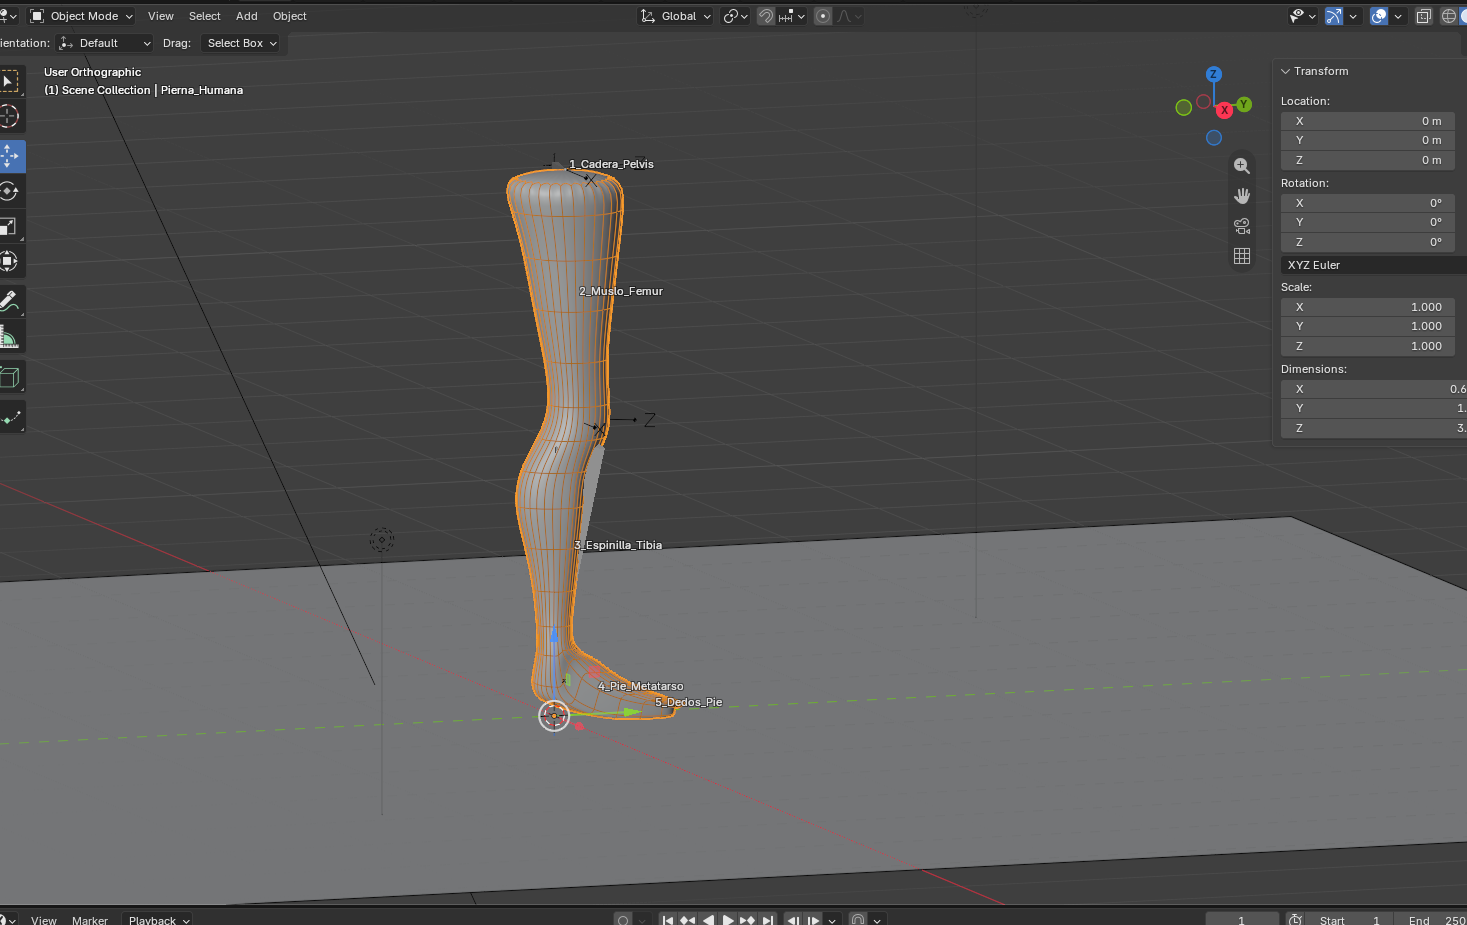
\includegraphics[width=0.55\textwidth]{Imagenes/E1/02_malla_topologia_alambre.png}
    \caption{Topología de la malla continua de la pierna en sombreado sólido con visualización de aristas (\textit{Wireframe}), apreciando la disposición de bucles cuadriláteros (\textit{quad loops}) alrededor de las zonas articulares.}
    \label{fig:exp_topologia}
\end{figure}

Una vez que la geometría estuvo lista, creamos una armadura básica insertando un solo hueso (\texttt{Shift + A} $\to$ \textit{Armature} $\to$ \textit{Single Bone}) para comenzar el sistema esquelético. Colocamos el primer hueso como raíz en la cadera (\texttt{1\_Cadera\_Pelvis}) y a partir de su extremo (\textit{tail}) fuimos extruyendo consecutivamente con la tecla \texttt{E} los cuatro huesos restantes: el fémur (\texttt{2\_Muslo\_Femur}), la espinilla (\texttt{3\_Espinilla\_Tibia}), el metatarso (\texttt{4\_Pie\_Metatarso}) y los dedos (\texttt{5\_Dedos\_Pie}), manteniendo siempre la opción \texttt{Connected} activa para que las articulaciones no se desfasaran ni se separaran al rotar. Para poder supervisar con claridad la armadura dentro del cuerpo, activamos las casillas \textit{In Front} (Rayos X) y \textit{Names} en las propiedades de visualización de Blender, tal como se muestra en la Figura \ref{fig:exp_armadura_rayosx} (izquierda).

Fue justo al colocar estos huesos donde nos topamos con nuestro primer problema importante. Al inicio habíamos colocado el fémur y la espinilla formando una línea vertical perfectamente recta ($180^\circ$). Sin embargo, al pasar a hacer las primeras pruebas de flexión, el cálculo de rotación no tenía un plano preferente y la rodilla tendía a doblarse hacia cualquier dirección indeterminada o de manera inversa. Para solucionar esto regresamos a Modo Edición y, mirando la pierna desde la vista lateral ortogonal (\textit{Numpad 3}), desplazamos la cabeza de la rodilla ligeramente hacia adelante sobre el eje $+Y$, tal como se ilustra en la Figura \ref{fig:exp_armadura_rayosx} (derecha). Este pequeño ajuste le dio una pre-flexión anatómica natural a la cadena ósea que eliminó la ambigüedad matemática y forzó a que la rodilla siempre se flexionara correctamente hacia atrás.

\begin{figure}[H]
    \centering
    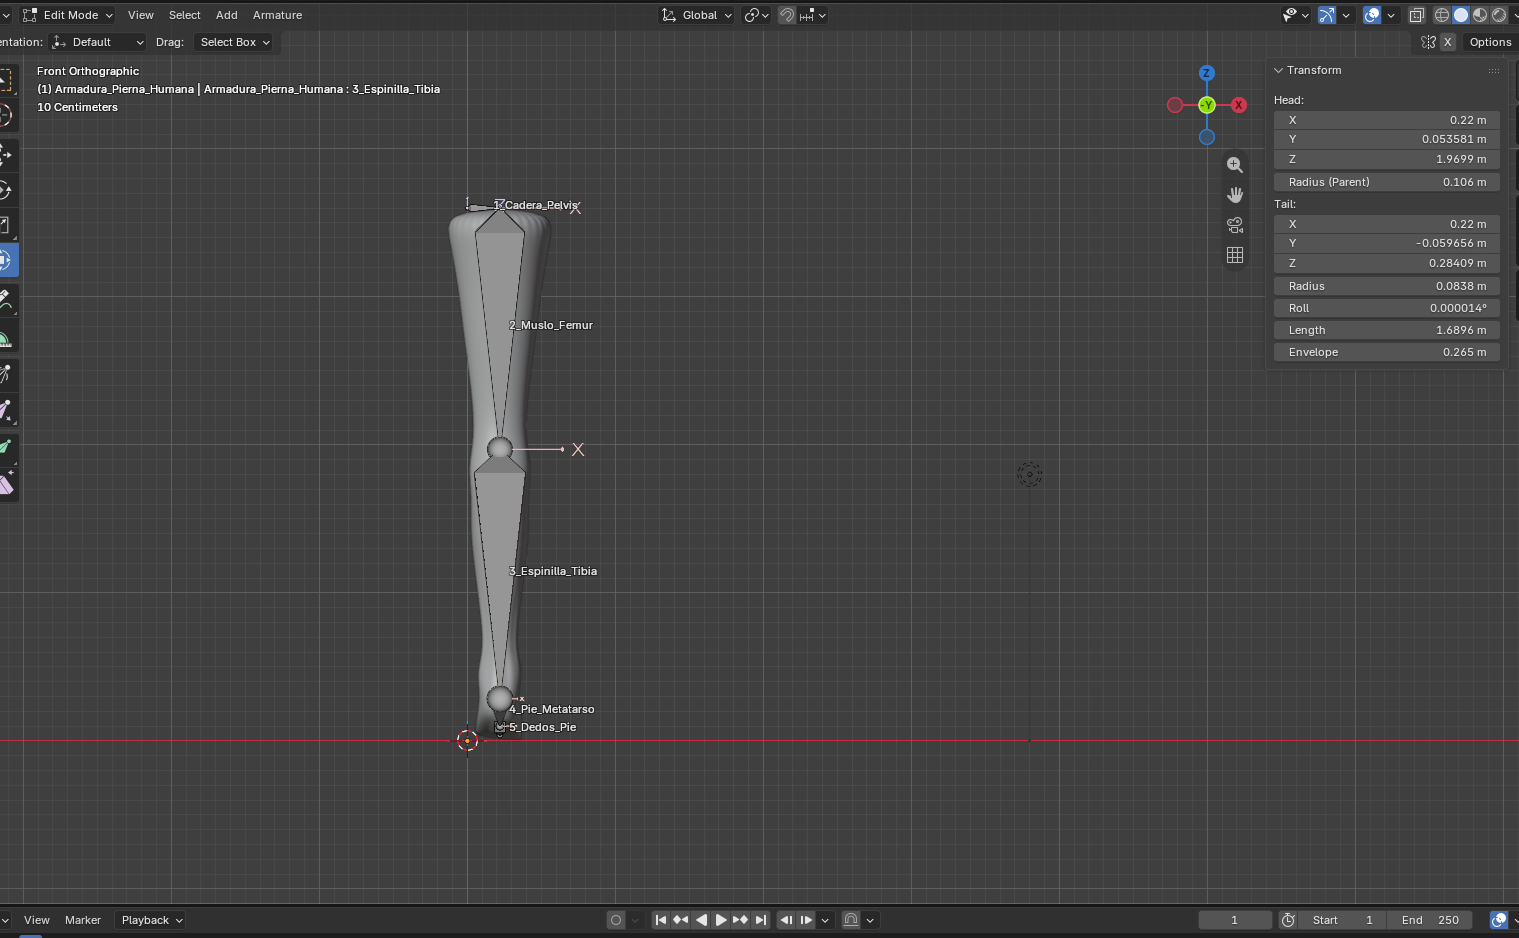
\includegraphics[width=0.45\textwidth]{Imagenes/E1/01_armadura_modo_edicion_rayosX.png}
    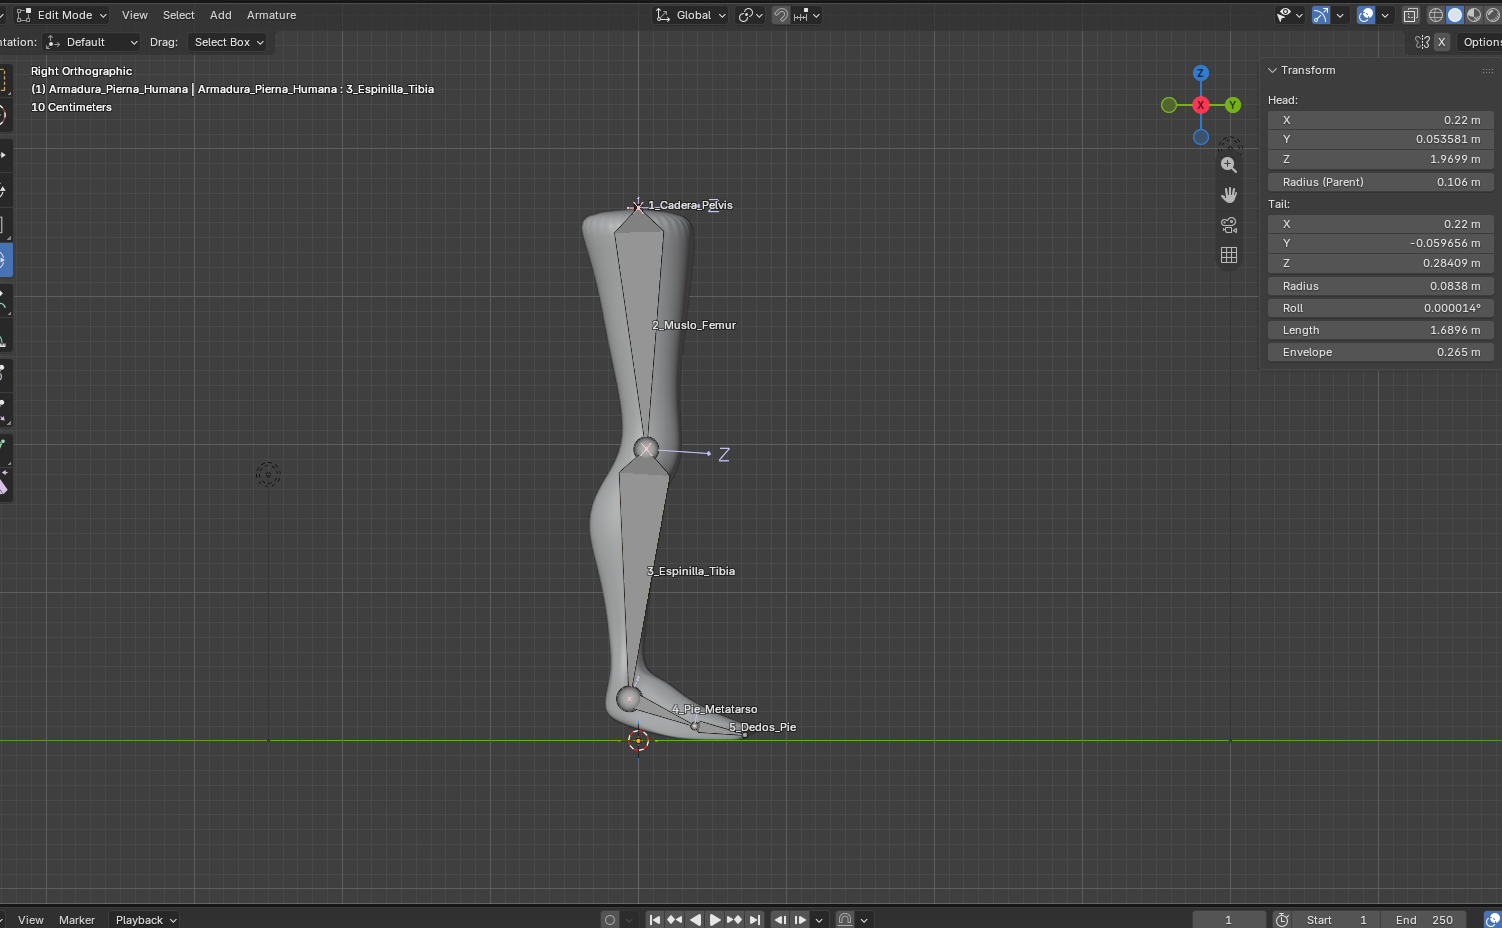
\includegraphics[width=0.45\textwidth]{Imagenes/E1/05_preflexion_rodilla_vista_lateral.png}
    \caption{Configuración de la armadura en Modo Edición: a la izquierda, cadena de 5 huesos con visualización de nombres y Rayos X (\textit{In Front}); a la derecha, vista lateral ortogonal mostrando la pre-flexión anterior ($+Y$) en la rodilla para definir el eje de rotación.}
    \label{fig:exp_armadura_rayosx}
\end{figure}

Con el esqueleto corregido procedimos a vincular la malla con la armadura. En Modo Objeto seleccionamos primero la pierna, luego la armadura con \texttt{Shift}, y aplicamos el atajo \texttt{Ctrl + P} seleccionando \textit{With Automatic Weights}. Esta operación asoció el modificador \textit{Armature} y generó los grupos de vértices de cada hueso mediante el algoritmo de difusión de calor de Blender. Para comprobar si los pesos se habían calculado de manera adecuada entramos a Modo Pintura de Pesos (\textit{Weight Paint}) y seleccionamos el fémur y la espinilla. Como se observa en la Figura \ref{fig:exp_weightpaint}, los bucles de soporte que habíamos previsto en el modelado permitieron que la influencia se distribuyera con un degradado térmico muy suave y progresivo en la rodilla, pasando gradualmente del rojo al azul sin transiciones bruscas, por lo que no fue necesario retocar pesos a mano.

\begin{figure}[H]
    \centering
    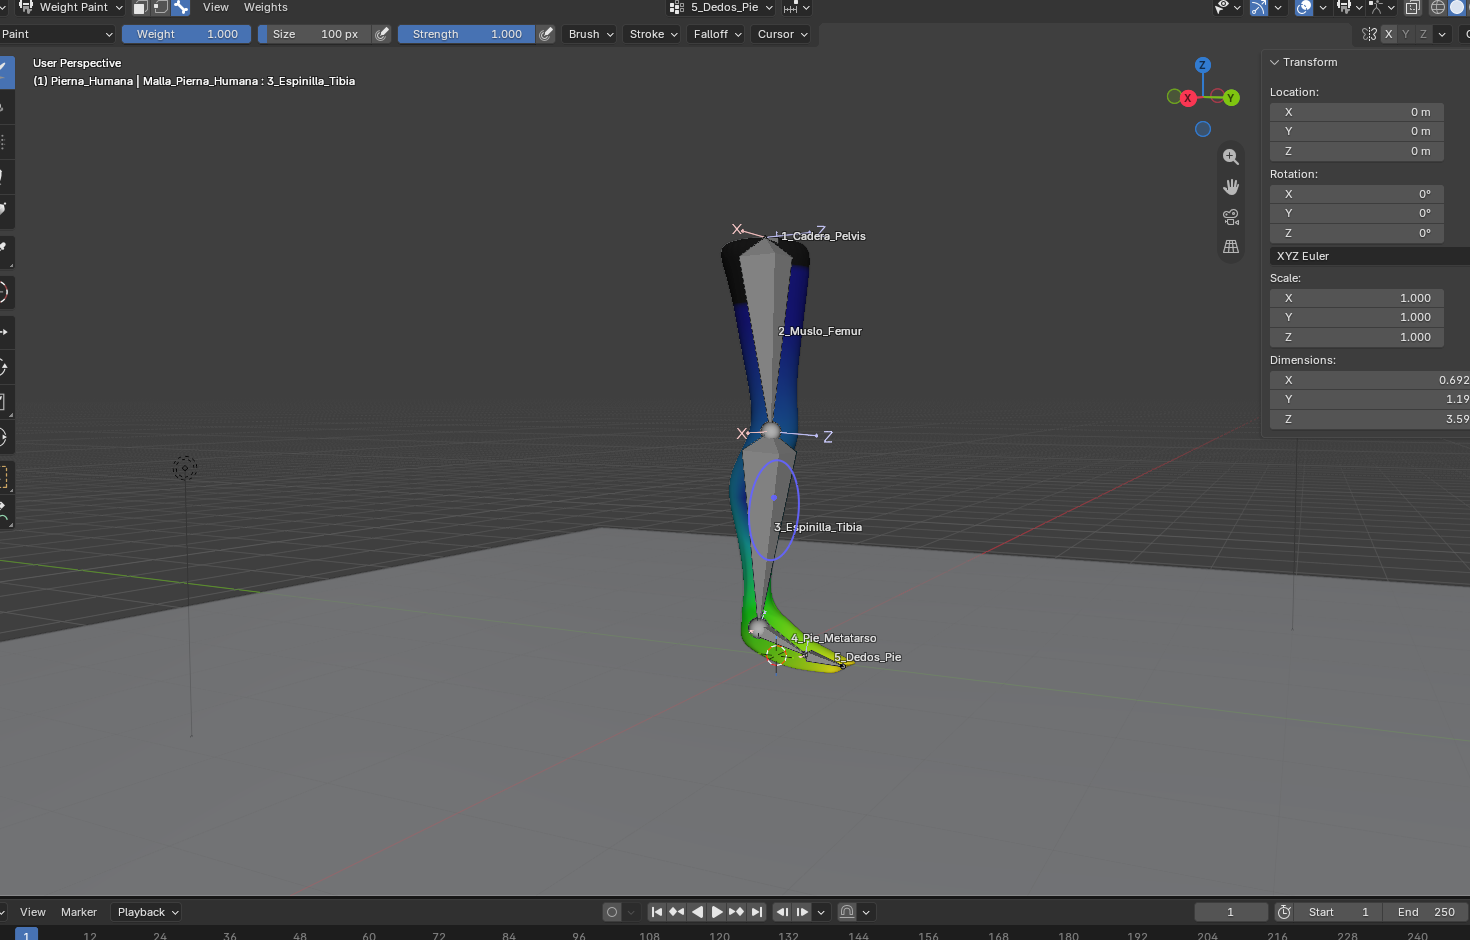
\includegraphics[width=0.55\textwidth]{Imagenes/E1/06_mapa_pesos_weight_paint_rodilla.png}
    \caption{Inspección en Modo Pintura de Pesos (\textit{Weight Paint}): degradado térmico de influencia en la rodilla generado automáticamente por el algoritmo de difusión de calor.}
    \label{fig:exp_weightpaint}
\end{figure}

Finalmente pasamos a Modo Pose (\texttt{Ctrl + Tab}) para evaluar el movimiento mediante Cinemática Directa (FK), rotando cada articulación de forma individual con la tecla \texttt{R}. Aquí comprobamos la herencia jerárquica en cascada: rotar la cadera mueve toda la pierna, rotar el fémur arrastra la rodilla y el pie, y rotar el pie solo mueve los dedos. En estas pruebas observamos un segundo detalle experimental: al forzar la rodilla a una flexión pronunciada (más de $90^\circ$), la parte posterior de la corva (pliegue poplíteo) se comprimía de más y tendía a perder volumen. Lo resolvimos agregando dos cortes de bucle adicionales con \texttt{Ctrl + R} alrededor de la rótula y el pliegue, lo que reforzó la densidad poligonal en esa zona y permitió que la pierna conservara su masa muscular incluso en ángulos de flexión cerrados.

\subsection{Actividad 2: Animación y análisis de relaciones padre-hijo de un personaje de Adobe Mixamo en Blender}
% [Pendiente de desarrollo]

\subsection{Actividad 3: Diagrama de las relaciones padre-hijo de la estructura jerárquica desde el nodo raíz}
% [Pendiente de desarrollo]

\subsection{Actividad 4: Exploración de software para estructuras humanoides (MakeHuman y DAZ3D)}
% [Pendiente de desarrollo]